
\chapter{A simple two parameter distribution for modelling neuronal activity and capturing neuronal association}

\label{chap:comb}

\subAbstract{Recent developments in electrophysiological technology have lead to an increase in the size of electrophysiology datasets. Consequently, there is a requirement for new analysis techniques that can make use of these new datasets, while remaining easy to use in practice. In this work, we fit some one or two parameter probability distributions to spiking data collected from a mouse exposed to visual stimuli. We show that the Conway-Maxwell-binomial distribution is a suitable model for the number of active neurons in a neuronal ensemble at any given moment. This distribution fits these data better than binomial or beta-binomial distributions. It also captures the correlated activity in the primary visual cortex induced by stimulus onset more effectively than simply measuring the correlations, at short timescales ($<10$ms). We also replicate the finding of Churchland et al (2010) relating to stimulus onset quenching neural variability in cortical areas, and we show a correspondence between this quenching and changes in one of the parameters of the fitted Conway-Maxwell-binomial distributions.}

\section{Introduction}
Recent advances in electrophysiological technology, such as `Neuropixels' probes \parencite{jun} have allowed extracellular voltage measurements to be collected from larger numbers of cells than traditional methods, in multiple brain regions simultaneously, and routinely. These larger datasets require innovative methods to extract information from the data in a reasonable amount of time, `reasonable' being subjective in this case.

Theoretically, all the information at any given moment in an electrophysiological dataset with $n$ neurons could be captured by calculating the probability distribution for every possible spiking pattern. This would require defining a random variable with $2^n$ possible values, a task that quickly becomes impossible as $n$ increases. Attempts at approximating this random variable often involve measuring pairwise or higher order correlations  \parencite{schneidman, flach, ganmor}. But pairwise correlations may not be enough to characterise instantaneous neural activity \parencite{tkacik}. Furthermore, these kinds of models tend to ignore the temporal structure of neuronal data, in favour of smaller model size, and scalability.

Higher order correlations would be helpful here, but defining and quantifying these correlations can be tricky \parencite{staude}. If we use the interaction parameters arising from the exponential family model as measures of higher order correlations, measuring these correlations becomes computationally impractical quite quickly (the number of `three neuron correlations' to measure scales with $\binom{n}{3}$). In this work, we dispense with measuring correlations directly, and we attempt to characterise correlated behaviour using a parameter in statistical model.

In this work, we examined the ability of simple distributions to model the number of active (spiking) neurons in a neuronal ensemble at any given timepoint. We compared a little-known distribution named the Conway-Maxwell-binomial distribution to the binomial distribution and the beta-binomial distribution. The binomial distribution is a probability distribution over the number of successes is a sequence of independent and identical Bernoulli trials. The beta-binomial distribution is similar, but allows for a bit more flexibility while still being a model for heterogeneity. Similar to the binomial and beta-binomial, the Conway-Maxwell-binomial distribution is a probability distribution over the number of successes in a series of Bernoulli trials, but allows over- and under-dispersion relative to the binomial distribution. This distribution should therefore be a good candidate for our purposes. We found that Conway-Maxwell-binomial distribution was usually the best candidate of the three that we examined.

We also observed some interesting changes in the number of active neurons in the primary visual cortex and hippocampus at stimulus onset and some changes in this activity in the thalamus which were sustained for the full duration of the stimulus presentation. This let us know that there were some responses to model.

We found that fitting a Conway-Maxwell-binomial distribution was a better method of capturing association between neurons than measuring the spike count correlation for the short time bins that we used ($<10$ms).

Finally, we also wanted to investigate parallels between the parameters of the Conway-Maxwell-binomial distribution and quantities that have been established as relevant to sensory processing. So, we replicated the findings made by Churchland et al. (2010) relating to a reduction in neural variability at stimulus onset in the macaque cortical regions, but for data taken from the mouse primary visual cortex. We compared these findings to the values of the fitted Conway-Maxwell-binomial distribution parameters.

\section{Data}
We used data collected by Nick Steinmetz and his lab `CortexLab at UCL'  \parencite{steinmetz}. The data can be found online \footnote{\url{http://data.cortexlab.net/dualPhase3/}} and are free to use for research purposes.

Two `Phase3' Neuropixels  \parencite{jun} electrode arrays were inserted into the brain of an awake, head-fixed mouse for about an hour and a half. These electrode arrays recorded $384$ channels of neural data each at $30$kHz and  less than $7\mu$V RMS noise levels. The sites are densely spaced in a `continuous tetrode'-like arrangement, and a whole array records from a $3.8$mm span of the brain. One array recorded from visual cortex, hippocampus,  and thalamus, the other array recorded from motor cortex and striatum. The data were spike-sorted automatically by Kilosort and manually by Nick Steinmetz using Phy. In total 831 well-isolated individual neurons were identified.

  \subsection{Experimental protocol}\label{sec:experimental_protocal}
  The mouse was shown a visual stimulus on three monitors placed around the mouse at right angles to each other, covering about $\pm 135$ degrees azimuth and $\pm 35$ degrees elevation.

  The stimulus consisted of sine-wave modulated full-field drifting gratings of 16 drift directions ($0^{\circ}, 22.5^{\circ}, \dots, 337.5^{\circ}$) with $2$Hz temporal frequency and $0.08$ cycles/degree spatial frequency displayed for $2$ seconds plus a blank condition. Each of these $17$ conditions were presented $10$ times in a random order across $170$ different trials. There were therefore $160$ trials with a drifting-grating visual stimulus present, and $10$ trials with a blank stimulus.

\section{Methods}

    \subsection{Binning data}
    We converted the spike times for each cell into spike counts by putting the spike times into time bins of a given `width' (in milliseconds). We used time bins of $1$ms, $5$ms, and $10$ms. We used different time bin widths to assess the impact of choosing a bin width.


    \subsection{Number of \textit{active} neurons}\label{sec:num_active_neurons}
    To count the number of active neurons in each neuronal ensemble, we split the time interval for each trial into bins of a given width. We counted the number of spikes fired by each cell in each bin. If a cell fired \textit{at least} one spike in a given bin, we regarded that cell as active in that bin. We recorded the number of active cells in every bin, and for the purposes of further analysis, we recorded each cell's individual spike counts.

    It should be noted that when we used a bin width of $1$ms, the maximum number of spikes in any bin was $1$. For the wider time bins, some bins had spike counts greater than $1$. Consequently when using a bin width of $1$ms, the number of active neurons and the total spike count of a given bin were identical. But for wider bin widths, the total spike count was greater than the number of active neurons.

    So for the $1$ms bin width, the activity of a neuron and the number of spikes fired by that neuron in any bin can be modelled as a Bernoulli variable. But for wider time bins, only the activity can be modelled in this way.

    \subsection{Moving windows for measurements}

    When taking measurements (e.g. moving average over the number of active neurons) or fitting distributions (eg. the beta binomial distribution) we slid a window containing a certain number of bins across the data, and made our measurements at each window position. For example, when analysing $1$ms bin data, we used a window containing $100$ bins, and we slid the window across the time interval for each trial moving $10$ bins at a time. So that for $3060$ms of data, we made $296$ measurements.

    For the $5$ms bin width data, we used windows containing $40$ bins, and slid the window $2$ bins at a time when taking measurements.

    For the $10$ms bin width data, we used windows containing $40$ bins, and slid the window $1$ bin at a time when taking measurements (see table \ref{tab:bin_widths} for concise details).

    By continuing to use windows containing $40$ bins, we retained statistical power but sacrificed the number of measurements taken.

    \begin{table}
      \centering
      \begin{tabular}[h]{|c|c|c|c|}
        \hline
        \textbf{Bin width (ms)}   & \textbf{Window size (bins)}   & \textbf{Window size (ms)} & \textbf{Windows per trial}  \\ \hline
        $1$ms                     & $100$                         & $100$ms                   & $296$                       \\ \hline
        $5$ms                     & $40$                          & $200$ms                   & $286$                       \\ \hline
        $10$ms                    & $40$                          & $400$ms                   & $266$                       \\ \hline
      \end{tabular}
      \caption{Details of the different bin width and analysis window sizes used when binning spike times, and analysing those data.}
      \label{tab:bin_widths}
    \end{table}

    There was an interval between each trial with a grey image in place of the moving of the moving bar stimulus. This interval varied in time. But we included some of this interval when recording the data for each trial. We started recording the number of active neurons, and the number of spikes from each neuron from $530$ms before each trial until $1030$ms after each trial. This way, we could see the change in our measurements at the onset of a stimulus and the end of stimulus presentation.

    As mentioned in section \ref{sec:num_active_neurons}, we recorded the number of active neurons in each bin, and the spike count for each neuron in each bin. The actual measurements we took using these data in each window were as follows:
    \begin{description}
      \item[Moving average] The average number of active cells in each window.
      \item[Moving variance] The variance of the number of active cells in each window.
      \item[Average correlation] We measured the correlation between the spike counts of each pair of cells in the ensemble, and took the average of these measurements.
      \item[Binomial \textit{\textbf{p}}] We fitted a binomial distribution to the data in each window and recorded the fitted probability of success, $p$ in each case.
      \item[Beta-binomial $\boldsymbol{\alpha}$, $\boldsymbol{\beta}$] We fitted a beta-binomial distribution to the data in each window, and recorded the values of the fitted shape parameters, $\alpha$ and $\beta$, of each distribution.
      \item[Conway-Maxwell-binomial distribution \textit{\textbf{p}}, $\boldsymbol{\nu}$] We fitted a Conway-Maxwell-binomial distribution to the data in each window, and recorded the fitted values of $p$ and $\nu$ for each distribution.
      \item[Log-likelihoods] We also recorded the log-likelihood of each of the fitted distributions for each window.
    \end{description}

    \subsection{Fano factor}\label{sec:fano_factor}
    The \textit{Fano factor} of a random variable is defined as the ratio of the variable's variance to its mean.
    \begin{align}\label{eq:fano_factor}
      F = \frac{\sigma^2}{\mu}
    \end{align}
    We measured the Fano factor of the spike count of a given cell by measuring the mean and variance of the spike count across trials, and taking the ratio of those two quantities. When calculated in this way the Fano factor can be used as a measure of neural variability that controls for changes in the firing rate.  This is similar to the calculation used in \parencite{Churchland}.

    \subsection{Probability Distributions suitable for modelling ensemble activity}

    We present here three different probability distributions that could be suitable to model the number of active neurons in an ensemble. Each distribution has the set $\lbrace 0, \dots, n \rbrace$ as its support, where $n$ is the number of neurons in the ensemble. These are simple distributions with either two or three parameters each. However, we regard $n$ as known when using these distributions for modelling, so in effect each distribution has either one or two free parameters.

      \subsubsection{Association}\label{sec:association}
      \textit{Association} between random variables is similar to the correlation between random variables but is more general in concept. The correlation coefficient is a measure of association; and association doesn't necessarily have a mathematical definition like correlation does. Essentially, an association between two random variables is a dependency of any kind. Positively associated variables tend to take the same value, and negatively associated variables tend to take different values. In this research, we work with probability distributions of the number of successes in a set of Bernoulli trials. These Bernoulli variables may or may not be associated.

      A probability distribution over the number of successes in $n$ Bernoulli trials, where the Bernoulli variables may be associated, could constitute a good model for the number of active neurons in an ensemble of $n$ neurons. As long as the observation period is divided into time bins short enough so that any neuron is unlikely to fire more than spike in any time bin.

      \subsubsection{Binomial distribution}
      The binomial distribution is a two parameter discrete probability distribution that can be thought of as a probability distribution the number of successes from $n$ independent Bernoulli trials, each with the same probability of success. The parameters of the binomial distribution are $n$ the number of trials, and $0 \leq p \leq 1$, the probability of success for each of these trials. A random variable with the binomial distribution can take values from $\lbrace 0, \dots, n \rbrace$. The probability mass function of the distribution is
      \begin{align}\label{eq:binomial_pmf}
        P(k;n,p) = \binom{n}{k} p^k (1-p)^{n-k}
      \end{align}

      %%%%%%%%%% MAY REMOVE THIS PART %%%%%%%%%%%%%%
      % If we have $N$ independent samples from a binomial distribution and we know $n$ but want to estimate $p$, we can maximise the log likelihood function
      % \begin{align}\label{eq:binomial_log_like}
      %   L(p) & = \log P(\lbrace k_1, \dots, k_N \rbrace; n,p) \\
      %       & = \sum_{i=1}^N \log \binom{n}{k_i} + k_i \log p + (n-k_i)\log(1-p)
      % \end{align}

      % If we do not know $n$ there is no closed form way way of maximising this equation. Therefore the binomial distribution is generally only used in cases where we do know $n$. Consequently, the distribution is practically a one parameter distribution.
      %%%%%%%%%%%%%%%%%%%%%%%%%%%%%%%%%%%%%%%%%%%%%%

      As a model for the activity of a neuronal ensemble, the main problem with the binomial distribution is that it treats each neuron, represented as a Bernoulli trial, as independent. It is well know that neurons are not independent, and that correlated behaviour between neurons is vital for representing sensory information \parencite{cohen1}. The binomial distribution falls short in this regard, but it is useful as performance benchmark when assessing the performance of other models.

      \subsubsection{Beta-binomial distribution}
      The beta distribution is the conjugate distribution of the binomial distribution. The beta-binomial distribution is the combination of the beta distribution and the binomial distribution, in that the probability of success for the binomial distribution is sampled from the beta distribution. This allows the beta-binomial distribution to capture some over dispersion relative to the binomial distribution.

      The beta-binomial distribution is a three parameter distribution, $n$ the number of Bernoulli trials, and $\alpha \in \mathbb{R}_{>0}$ and $\beta \in \mathbb{R}_{>0}$ the shape parameters of the beta distribution. The probability mass function for the beta-binomial distribution is
      \begin{align}\label{eq:betabinomial_pdf}
        P(k;n, \alpha, \beta) = \binom{n}{k}\frac{B(k + \alpha, n - k + \beta)}{B(\alpha, \beta)}
      \end{align}
      where $B(\alpha, \beta)$ is the beta function.

      This probability distribution can be reparametrised in a number of ways. One of which defines new parameters $\pi$ and $\rho$ by
      \begin{align}\label{eq:betabinomial_reparam}
        \pi &= \frac{\alpha}{\alpha + \beta} \\
        \rho &= \frac{1}{\alpha + \beta + 1}
      \end{align}
      This reparametrisation is useful because $\pi$ acts as a location parameter analogous to the $p$ parameter of a binomial distribution. A value of $\rho > 0$ indicates over-dispersion relative to a binomial distribution.

      As a model for the activity of a neuronal ensemble, the beta-binomial distribution is more suitable than a binomial distribution because the over-dispersion of the beta-binomial distribution can be used to model positive association between the neurons. An extreme example of this over-dispersion/positive association can be seen in figure \ref{fig:betabinomial_big_overdispersion}. In this figure, the neurons are positively associated and so tend to take the same value, consequently the probability mass of the beta-binomial distribution builds up close to $k=0$ and $k=n$. It is worth noting that the location parameter for each distribution has the same value, $p=\pi=0.5$.

      \begin{figure}[h]
        \begin{subfigure}[h]{0.5\linewidth}
          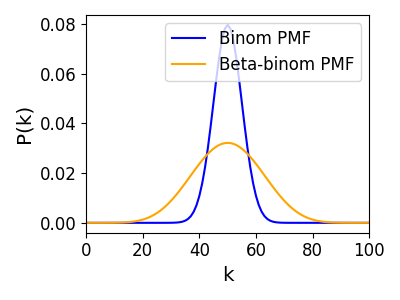
\includegraphics[width=\textwidth]{figures/conway_maxwell/betabinomial_overdispersion.png}
          \caption{$n=100, p=0.5, \alpha=\beta=10$}
          \label{fig:betabinomial_overdispersion}
        \end{subfigure}
        \begin{subfigure}[h]{0.5\linewidth}
          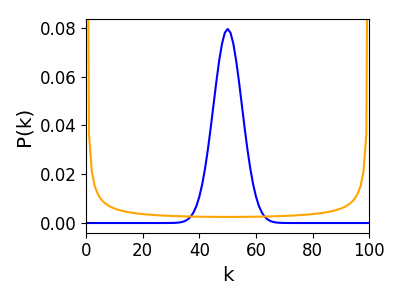
\includegraphics[width=\textwidth]{figures/conway_maxwell/betabinomial_big_overdispersion.png}
          \caption{$n=100, p=0.5, \alpha=\beta=0.3$}
          \label{fig:betabinomial_big_overdispersion}
        \end{subfigure}
        \caption{Figures showing the over-dispersion possible for a beta-binomial distribution relative to a binomial distribution. Parameters are shown in the captions. }
      \end{figure}

      \subsubsection{Conway-Maxwell-binomial distribution}\label{sec:conway_maxwell_binomial_distribution}
      The Conway-Maxwell-binomial distribution (COMb distribution) is a three parameter generalisation of the binomial distribution that allows for over dispersion and under dispersion relative to the binomial distribution. The parameters of the distribution are $n$ the number of Bernoulli trials, and two shape parameters $0 \leq p \leq 1$, and $\nu \in \mathbb{R}$.

      The probability mass function of the COMb distribution is
      \begin{align}\label{eq:comb_pmf}
        P(k;n,p,\nu) = \frac{1}{S(n,p,\nu)}\binom{n}{k}^{\nu} p^k (1-p)^{n-k}
      \end{align}
      where
      \begin{align}\label{eq:comb_norm}
        S(n,p,\nu) = \sum_{j=0}^n \binom{n}{k}^{\nu} p^j (1-p)^{n-j}
      \end{align}
      The only difference between this PMF and the PMF for the standard binomial is the introduction of $\nu$ and the consequent introduction of the normalising function $S(n,p,\nu)$.

      Indeed, if $\nu = 1$ the COMb distribution is identical to the binomial distribution with the same values for $n$ and $p$. We can see in figure \ref{fig:comb_bin_dkl} that the KL-divergence $D_{KL}(P_{COMb}(n,p,\nu) || P_{Bin}(n,p))=0$ along the line where $\nu=1$. The analytical expression for the divergence is
      \begin{align}
        D_{KL}(P_{COMb}(k;n,p,\nu) || P_{Bin}(k;n,p)) = &(\nu - 1) E_{P_{COMb}(k;n,p,\nu)}\left[ \log \binom{n}{k} \right] \\
          &- \log S(n,p,\nu)
      \end{align}
      At $\nu = 1$, we have $S(n,p,1)$ which is just the sum over the binomial PMF, so $S(n,p,1) = 1$ and therefore $D_{KL}(P_{COMb}(n,p,\nu) || P_{Bin}(n,p))=0$.

      If $\nu < 1$ the COMb distribution will exhibit over-dispersion relative to the binomial distribution. If $p=0.5$ and $\nu=0$ the COMb distribution is the discrete uniform distribution, and if $\nu < 0$ the mass of the COMb distribution will tend to build up near $k=0$ and $k=n$. This over-dispersion represents positive association in the Bernoulli variables. An example of this over-dispersion can be seen in figure \ref{fig:comb_overrdispersion}.

      If $\nu > 1$ the COMb distribution will exhibit under-dispersion relative to the binomial distribution. The larger the value of $\nu$ the more probability mass will build up at $n/2$ for even $n$, or at $\lfloor n/2 \rfloor$ and $\lceil n/2 \rceil$ for odd $n$. This under-dispersion represents negative association in the Bernoulli variables. An example of this under-dispersion can be seen in figure \ref{fig:comb_underdispersion}.

      It should be noted that the $p$ parameter of the COMb distribution does not correspond to the mean of the distribution, as is the case for the binomial $p$ parameter, and beta-binomial $\pi$ parameter. That is, the COMb $p$ parameter is not a location parameter. An illustration of this can be seen in figure \ref{fig:comb_skewed}. This is because an interaction between the $p$ and $\nu$ parameters skews the mean. There is no analytical expression for the mean of the COMb distribution.

      \begin{table}
        \centering
        \begin{tabular}[h]{|c|c|c|}
          \hline
          $\boldsymbol{\nu}$  & \textbf{Relative dispersion}  & \textbf{Association between neurons/variables} \\ \hline
          $<1$                & over                          & positive                                      \\ \hline
          $1$                 & none                          & none                                          \\ \hline
          $>1$                & under                         & negative                                      \\ \hline
        \end{tabular}
        \caption{Relative dispersion of the COMb distribution, and association between Bernoulli variables as represented by the value of the $\nu$ parameter.}
      \end{table}


      Since the COMb distribution has the potential to capture positive and negative associations between the neurons/Bernoulli variables, it should be an excellent candidate for modelling the number of active neurons in a neuronal ensemble.

      We wrote a dedicated Python package to enable easy creation and fitting of COMb distribution objects. The format of the package imitates the format of other distribution objects from the \texttt{scipy.stats} Python package. The COMb package can be found here: \\
      \url{https://github.com/thomasjdelaney/Conway_Maxwell_Binomial_Distribution}

      \begin{figure}[p]
        \begin{subfigure}[h]{0.5\linewidth}
          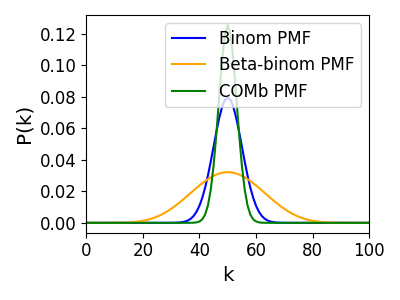
\includegraphics[width=\textwidth]{figures/conway_maxwell/comb_underdispersion.png}
          \caption{$n=100, p=0.5, \alpha=\beta=10, \nu=2.5$}
          \label{fig:comb_underdispersion}
        \end{subfigure}
        \begin{subfigure}[h]{0.5\linewidth}
          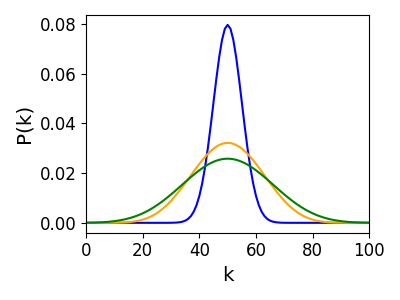
\includegraphics[width=\textwidth]{figures/conway_maxwell/comb_overrdispersion.png}
          \caption{$n=100, p=0.5, \alpha=\beta=0.3, \nu=0.1$}
          \label{fig:comb_overrdispersion}
        \end{subfigure}
        \begin{subfigure}[h]{0.5\linewidth}
          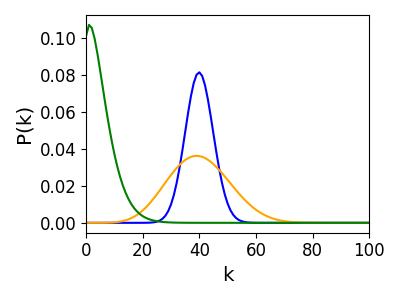
\includegraphics[width=\textwidth]{figures/conway_maxwell/comb_skewed.png}
          \caption{$n=100, p=0.4, \alpha=10, \beta=15, \nu=0.1$}
          \label{fig:comb_skewed}
        \end{subfigure}
        \begin{subfigure}[h]{0.5\linewidth}
          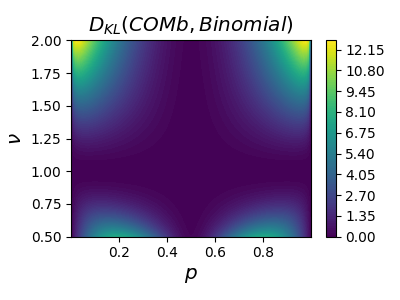
\includegraphics[width=\textwidth]{figures/conway_maxwell/comb_bin_dkl.png}
          \caption{KL-Divergence as a function of $p$ and $\nu$. $n=100$.}
          \label{fig:comb_bin_dkl}
        \end{subfigure}
        \caption{Figures showing (A) the under-dispersion and (B) over-dispersion permitted by the COMb distribution relative to a binomial distribution. (C) illustrates that the $p$ parameter of the COMb distribution does not correspond to the mean of the distribution, as it does for the binomial and beta-binomial distributions. (D) shows a heatmap for the value of the Kullback-Liebler divergence between the COMb distribution and the standard binomial distribution with same value for $n$, as a function of $p$ and $\nu$. Parameters are shown in the captions.}
      \end{figure}

    \subsection{Fitting}
    We fitted binomial, beta-binomial, and Conway-Maxwell-binomial (COMb) distributions to the neural activity in each of the overlapping windows covering each trial. To fit the distributions we minimised the appropriate negative log likelihood function using the data from the window.

    There is an analytical solution for maximum likelihood estimate of the binomial distribution's $p$ parameter.
    \begin{align}\label{eq:binomial_log_like_p_estimate}
      \hat{p} = \frac{1}{n}\sum_{i=1}^N k_i
    \end{align}

    We minimised the negative log likelihood function of the beta-binomial distribution numerically. We calculated the negative log likelihood for a sample directly, by taking the sum of the log of the probability mass function for each value in the sample. We minimised the negation of that function using the \texttt{minimise} function of the \texttt{scipy.optimize} Python package.

    The log likelihood function of the COMb distribution given some sample \\ $\lbrace k_1, \dots, k_N \rbrace$ is
    \begin{align}\label{eq:comb_log_like}
      \ell (p,\nu | k_1,\dots,k_N) =& N\left[n\log(1-p) - \log S(n,p,\nu)\right]  \\
        &+ \log \frac{p}{1-p} \sum_{i=1}^N k_i \\
        &+ \nu \sum_{i=1}^N \log \binom{n}{k_i}
    \end{align}
    We minimised the negation of this function using numerical methods. More specifically, we used the \texttt{minimise} function of the \texttt{scipy.optimize} Python package.

    \subsection{Goodness-of-fit}
    After fitting, we measured the goodness-of-fit of each model/distribution with their log likelihood. We calculated this directly using the \texttt{logpmf} functions of the distribution objects in Python.

\section{Results}
We defined a neuron as \textit{active} in a time bin if it fires at least one spike during the time interval covered by that bin. We measured the number of active neurons in the primary visual cortex of a mouse in $1$ms bins across $160$ trials of a moving bar visual stimulus. We then slid a $100$ms window across these $1$ms bins taking measurements, and fitting distributions along the way. We did the same for neurons in the thalamus, hippocampus, striatum, and motor cortex. We repeated the analysis for $5$ms time bins with $40$ bin windows, and $10$ms time bins with $40$ bin windows.

  \subsection{Increases in mean number of active neurons and variance in number of active neurons at stimulus onset in some regions}
  We measured the average number of active neurons, and the variance of the number of active neurons in a $100$ms sliding window starting $500$ms before stimulus onset until $1000$ms after stimulus onset. We found differences in the response across regions. There were no observed changes in response to the stimulus in the motor cortex or the striatum. The changes in the other regions are detailed below.

    \subsubsection{Primary visual cortex}
    We found a transient increase in both the average and variance of the number of active neurons at stimulus onset, followed by a fall to pre-stimulus levels, followed by another transient increase (see figure \ref{fig:v1_moving_avg_and_var}). The oscillation in both of these measurements appear to reflect the frequency of the stimulus (see Data section \ref{sec:experimental_protocal}), and it is known that stimulus structure can influence response structure\parencite{litwinkumar}. We see a similar but lower amplitude oscillation at the end of the stimulus presentation.

    \begin{figure}[p]
      \begin{subfigure}[h]{\linewidth}
        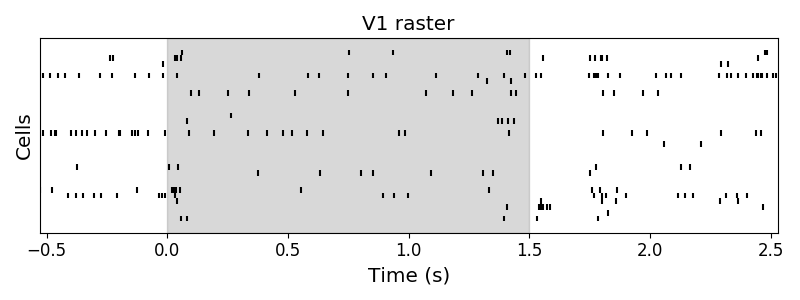
\includegraphics[width=\linewidth]{figures/conway_maxwell/v1_raster_16.png}
        \caption{Raster.}
        \label{fig:v1_raster}
      \end{subfigure}
      \begin{subfigure}[h]{\linewidth}
        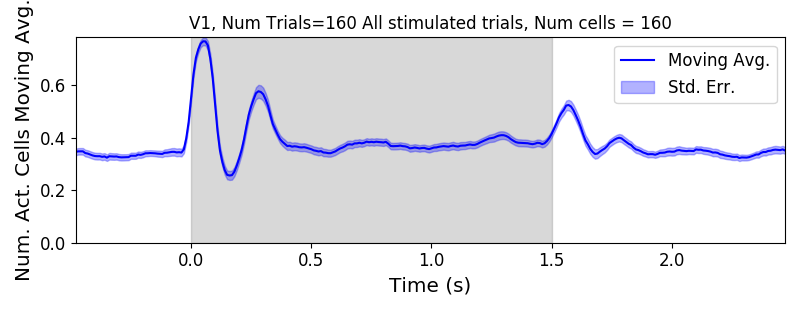
\includegraphics[width=\linewidth]{figures/conway_maxwell/v1_1ms_moving_avg_all_stimulated_trials.png}
        \caption{Moving average.}
        \label{fig:v1_moving_avg_num_active_cells}
      \end{subfigure}
      \begin{subfigure}[h]{\linewidth}
        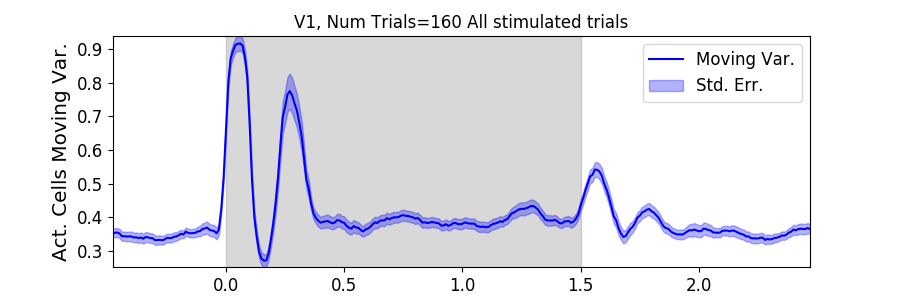
\includegraphics[width=\linewidth]{figures/conway_maxwell/v1_1ms_moving_var_all_stimulated_trials.png}
        \caption{Moving variance.}
        \label{fig:v1_moving_var_num_active_cells}
      \end{subfigure}
      \caption{(A) Raster plot showing the spikes fired by $33$ randomly chosen neurons in the primary visual cortex. (B-C) (B) average and (C) variance of the number of active neurons, measured using a sliding window $100$ms wide, split into $100$ bins. The midpoint of the time interval for each window is used as the timepoint (x-axis point) for the measurements using that window. The grey shaded area indicates the presence of a visual stimulus. The opaque line is an average across the $160$ trials that included a visual stimulus of any kind. We can see a transient increase in the average number of active neurons and the variance of this number, followed by a fluctuation and another increase.}
      \label{fig:v1_moving_avg_and_var}
    \end{figure}

    \subsubsection{Hippocampus}
    In the hippocampus we observed a transient increase in the average number of active neurons and in the variance of the number of active neurons at stimulus onset (see figure \ref{fig:hippocampus_moving_avg_and_var}). The increase lasted about $125$ms, and the subsequent fall to baseline took the a similar amount of time.

    \begin{figure}[p]
      \begin{subfigure}[h]{\linewidth}
        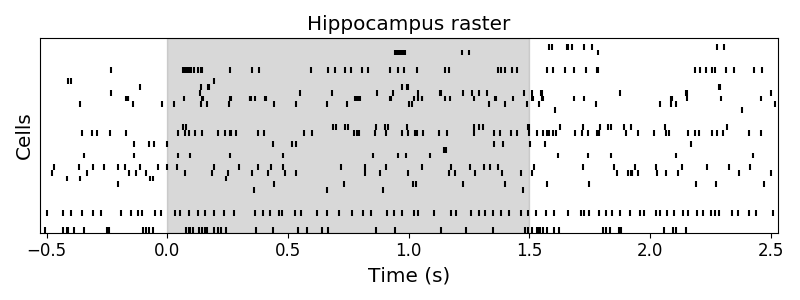
\includegraphics[width=\linewidth]{figures/conway_maxwell/hippocampus_raster_16.png}
        \caption{Raster.}
        \label{fig:hippocampus_raster}
      \end{subfigure}
      \begin{subfigure}[h]{\linewidth}
        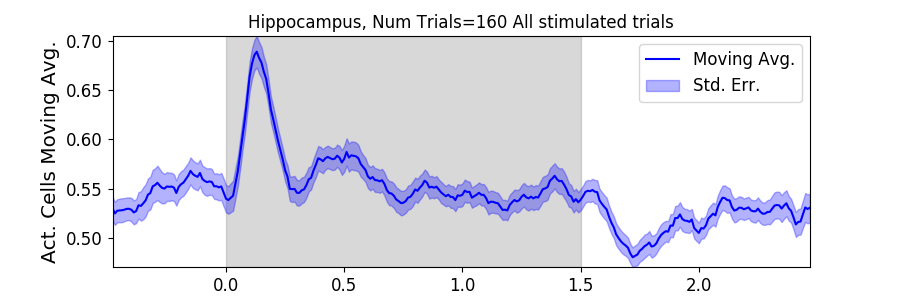
\includegraphics[width=\linewidth]{figures/conway_maxwell/hippocampus_1ms_moving_avg_all_stimulated_trials.png}
        \caption{Moving average.}
        \label{fig:hippocampus_moving_avg_num_active_cells}
      \end{subfigure}
      \begin{subfigure}[h]{\linewidth}
        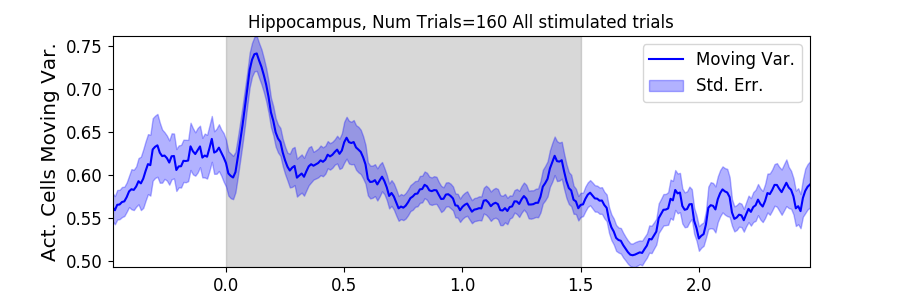
\includegraphics[width=\linewidth]{figures/conway_maxwell/hippocampus_1ms_moving_var_all_stimulated_trials.png}
        \caption{Moving variance.}
        \label{fig:hippocampus_moving_var_num_active_cells}
      \end{subfigure}
      \caption{(A) Raster plot showing the spikes fired by $33$ randomly chosen neurons in the hippocampus. (B-C) (B) average and (C) variance of the number of active neurons, measured using a sliding window $100$ms wide, split into $100$ bins. The midpoint of the time interval for each window is used as the timepoint (x-axis point) for the measurements using that window. The grey shaded area indicates the presence of a visual stimulus. The opaque line is an average across the $160$ trials that included a visual stimulus of any kind. We can see a transient increase in the average number of active neurons and the variance of this number at stimulus onset.}
      \label{fig:hippocampus_moving_avg_and_var}
    \end{figure}

    \subsubsection{Thalamus}
    In the thalamus we observed a transient increase in the both the average and variance of the number of active neurons on stimulus onset, followed by a fall to pre-stimulus levels, followed by a sustained increase until the stimulus presentation ends.

    \begin{figure}[p]
      \begin{subfigure}[h]{\linewidth}
        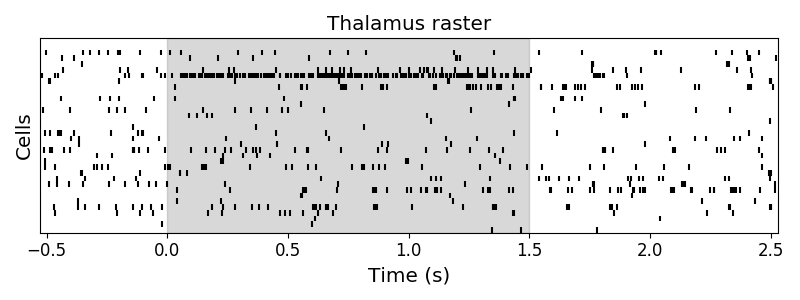
\includegraphics[width=\linewidth]{figures/conway_maxwell/thalamus_raster_16.png}
        \caption{Raster.}
        \label{fig:thalamus_raster}
      \end{subfigure}
      \begin{subfigure}[h]{\linewidth}
        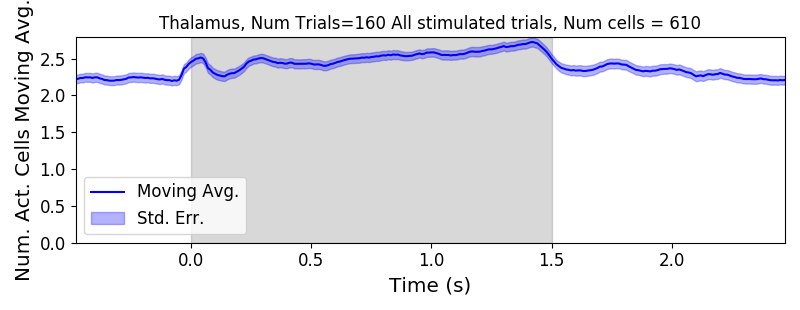
\includegraphics[width=\linewidth]{figures/conway_maxwell/thalamus_1ms_moving_avg_all_stimulated_trials.png}
        \caption{Moving average.}
        \label{fig:thalamus_moving_avg_num_active_cells}
      \end{subfigure}
      \begin{subfigure}[h]{\linewidth}
        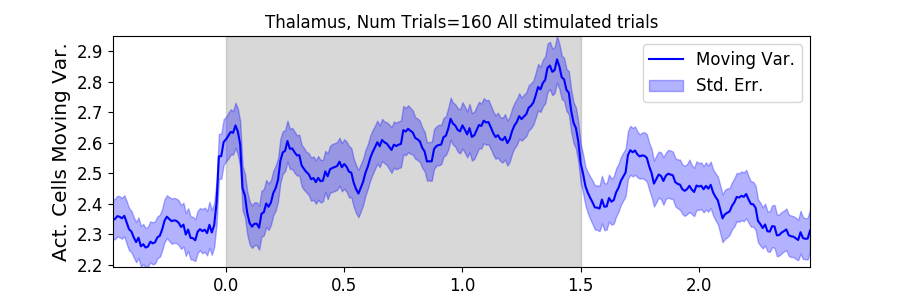
\includegraphics[width=\linewidth]{figures/conway_maxwell/thalamus_1ms_moving_var_all_stimulated_trials.png}
        \caption{Moving variance.}
        \label{fig:thalamus_moving_var_num_active_cells}
      \end{subfigure}
      \caption{(A) Raster plot showing the spikes fired by $33$ randomly chosen neurons in the thalamus. (B-C) (B) average and (C) variance of the number of active neurons, measured using a sliding window $100$ms wide, split into $100$ bins. The midpoint of the time interval for each window is used as the timepoint (x-axis point) for the measurements using that window. The grey shaded area indicates the presence of a visual stimulus. The opaque line is an average across the $160$ trials that included a visual stimulus of any kind. We can see in immediate increase at stimulus onset, a subsequent fall, and another sustained increased until the stimulus presentation ends.}
      \label{fig:thalamus_moving_avg_and_var}
    \end{figure}

    As one you might expect for a visual stimulus, the change in the average number of active neurons was greatest in the primary visual cortex. In this region, this quantity doubled on stimulus onset. In contrast, in the hippocampus and the thalamus, the average number of active neurons only increased by a fraction of the unstimulated baseline value. The duration of the response in V1 and the hippocampus at stimulus onset was $300-400$ms, but the response in the thalamus appeared to last for the duration of stimulus presentation. The V1 also showed a change in the average number of active neurons at stimulus end. The change was similar to that observed at stimulus onset, but smaller in magnitude (see figures \ref{fig:v1_moving_avg_and_var}, \ref{fig:hippocampus_moving_avg_and_var}, and \ref{fig:thalamus_moving_avg_and_var})

  \subsection{Conway-Maxwell-binomial distribution is usually a better fit than binomial or beta-binomial}
  Since the Conway-Maxwell-binomial distribution has not been fitted to neuronal data before, it is not clear that it would be a better fit than the binomial or beta-binomial distributions. In order to find out which parametric distribution was the best fit for the largest proportion of our data, we fit a binomial, a beta-binomial, and a Conway-Maxwell-binomial (COMb) distribution to each window for each bin width, and each region. Then we assessed the goodness-of-fit of each distribution by calculating the log-likelihood of each fitted distribution using the associated sample. We measured the proportion of samples for which each distribution was the best fit, for each bin width value and each region.

  We found that the COMb distribution was the best fit for most of the samples regardless of bin width or region. The bin width had an effect on the number of samples for which the COMb distribution was the best fit. The results are summarised in table \ref{tab:proportions}. For a bin width of $1$ms, the COMb distribution was the best fit for over $90\%$ of samples, the beta-binomial distribution was the best fit for less than $10\%$ of samples, and the binomial distribution was the best fit for less that $1\%$ of samples, across regions. For $5$ms bins, the COMb distribution was the best fit for $70-80\%$ of samples, the beta-binomial distribution was the best fit for $20-30\%$ of the samples, and again the binomial distribution was the best fit for less that $1\%$ of samples, across regions. Finally, for $10$ms bins,  the COMb distribution was the best fit for $53-80\%$ of samples, the beta-binomial distribution was the best fit for $20-47\%$ of the samples, and the binomial distribution was the best fit for less that $0.1\%$ of samples, across regions.

  \begin{figure}[h]
    \begin{subfigure}[h]{0.5\linewidth}
      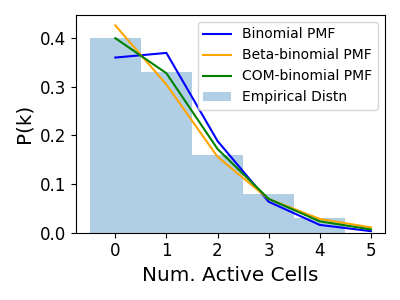
\includegraphics[width=\linewidth]{figures/conway_maxwell/fitting_example.png}
      \caption{Example of fitted distributions.}
      \label{fig:fitting_example}
    \end{subfigure}
    \begin{subfigure}[h]{0.5\linewidth}
      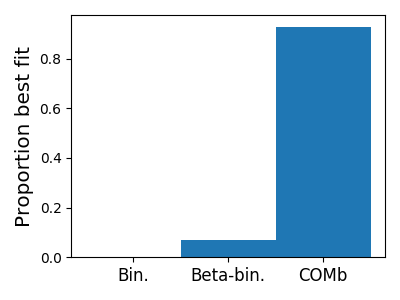
\includegraphics[width=\linewidth]{figures/conway_maxwell/best_fit_proportion.png}
      \caption{Proportion of best fit}
      \label{fig:best_fit_proportion}
    \end{subfigure}
    \caption{(A) An example of the binomial, beta-binomial, and Conway-Maxwell-binomial distributions fitted to a sample of neural activity. The Conway-Maxwell-binomial distribution is the best fit in this case. The histogram shows the empirical distribution of the sample. The probability mass function of each distribution is indicated by a different coloured line. (B) Across all samples in all trials, the proportion of samples for which each fitted distribution was the the best fit. The Conway-Maxwell-binomial distribution was the best fit for $93\%$ of the samples taken from V1 using a bin width of $1$ms.}
    \label{fig:fitting}
  \end{figure}

  \begin{table}
    \centering
    \begin{tabular}[h]{|c|c|c|c|}
      \hline
      \textbf{Bin Width (ms)} & \textbf{Binomial}  & \textbf{Beta-binomial} & \textbf{COMb}  \\ \hline
      $1$ms                   & $<1\%$                        & $<10\%$                           & $>90\%$                   \\ \hline
      $5$ms                   & $<0.1\%$                      & $20-30\%$                         & $70-80\%$                 \\ \hline
      $10$ms                  & $<0.1\%$                      & $20-47\%$                         & $53-80\%$                 \\ \hline
    \end{tabular}
    \caption{Proportion of samples for which each distribution was the best fit, grouped by bin width. The COMb distribution is the best fit most of the time.}
    \label{tab:proportions}
  \end{table}

  \newpage

  \subsection{Conway-Maxwell-binomial distribution captures changes in association at stimulus onset}
  We fit a Conway-Maxwell-binomial (COMb) distribution to the number of active neurons in the $1$ms time bins in a $100$ms sliding window. We also measured the correlation coefficient between the spike counts of all possible pairs of neurons, and took the average of these coefficients. We did this for all the trials with a visual stimulus. We observed a reduction in the COMb distribution's $\nu$ parameter at stimulus onset from around $1$ to between $0$ and $1$ (see figure \ref{fig:comb_nu_parameter}). A value of $\nu$ less than $1$ indicates positive association between the neurons (see section \ref{sec:conway_maxwell_binomial_distribution}). We might expect to see this positive association reflected in the correlation coefficients, but this is not the case. We see no change in the time series of average correlation measures at stimulus onset.

  This may be due to the very short time bin we used in this case. We know that using small time bins can artificially reduce correlation measurements  \parencite{cohen2}. In this case, fitting the COMb distribution may be a useful way to measure association in a neuronal ensemble over very short timescales ($<10$ms).

  \begin{figure}[h]
    \begin{subfigure}[h]{\linewidth}
      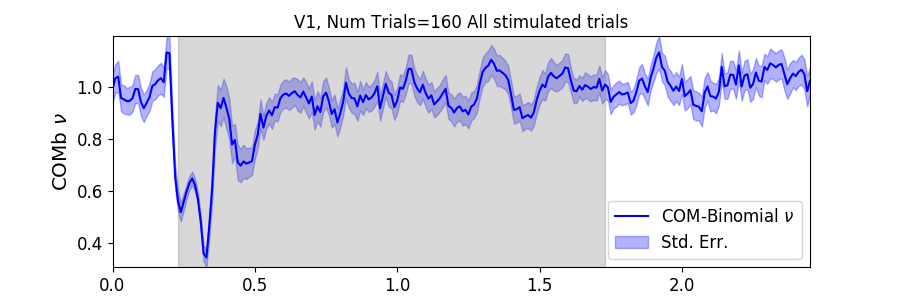
\includegraphics[width=\linewidth]{figures/conway_maxwell/v1_1ms_comb_nu_all_stimulated_trials.png}
      \caption{COMb $\nu$ parameter.}
      \label{fig:comb_nu_parameter}
    \end{subfigure}
    \begin{subfigure}[h]{\linewidth}
      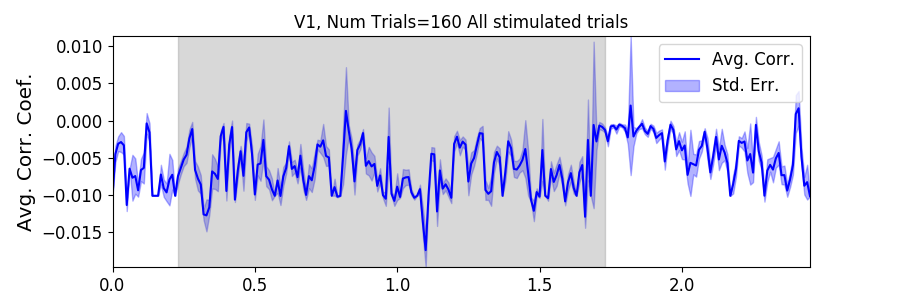
\includegraphics[width=\linewidth]{figures/conway_maxwell/v1_1ms_corr_avg_all_stimulated_trials.png}
      \caption{Average correlation coefficient.}
      \label{fig:avg_corr_coef}
    \end{subfigure}
    \caption{(A) We fit a Conway-Maxwell-binomial distribution to the number of active neurons in $1$ms time bins of a $100$ms sliding window. We did this for all trials with a visual stimulus and took the average across those trials. We see a transient drop in value for the distribution's $\nu$ parameter at stimulus onset. This shows an increase in positive association between the neurons. (B) We measured the correlation coefficient between the spike counts of all possible pairs of neurons in the same sliding window. The took the average of those coefficients. We also did this for every visually stimulated trial, and took the average across trials. The increase in positive association is not reflected with an increase in average correlation.}
    \label{fig:comb_nu_and_corr}
  \end{figure}

  \subsection{Replicating stimulus related quenching of neural variability}
  Churchland et al. (2010) inspected the effect of a stimulus on neural variability. One of the measures of neural variability that they employed was the Fano factor of the spike counts of individual cells (see section \ref{sec:fano_factor}). They found a reduction in neural variability as measured by the Fano factor in various cortical areas in a macaque at the onset of various visual stimuli, or a juice reward \parencite{Churchland}.

  We measured the Fano factor of the spike count of each cell in each brain region, during each trial. We measured the mean and standard error of these Fano factors from $500$ms before stimulus onset until $1000$ms after stimulus end. For the primary visual cortex, we found a transient reduction in the Fano factor immediately after stimulus onset. We used a Mann-Whitney U test to check that the Fano factors measured in a window starting at stimulus onset and ending $100$ms later were significantly lower than the factors measured in a window ending at stimulus onset ($p < 0.001$, see figure \ref{fig:v1_1ms_fano_factor}). We did not get this statistically significant result in any other region.

  Our findings agree with those of Churchland et al. for the primary visual cortex. However Churchland also found a reduction in the Fano factor in the dorsal premotor cortex (PMd) at stimulus onset. Our measurements from the mouse motor cortex show no change at stimulus onset (see figure \ref{fig:motor_cortex_fano_factor}). This could indicate some difference in the functionality of the motor cortex in a macaque and the motor cortex of a mouse.

  \begin{figure}[h]
    \begin{subfigure}[h]{0.5\linewidth}
      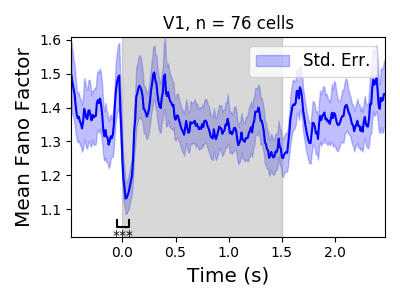
\includegraphics[width=\linewidth]{figures/conway_maxwell/v1_1ms_fano_factor.png}
      \caption{Primary visual cortex.}
      \label{fig:v1_1ms_fano_factor}
    \end{subfigure}
    \begin{subfigure}[h]{0.5\linewidth}
      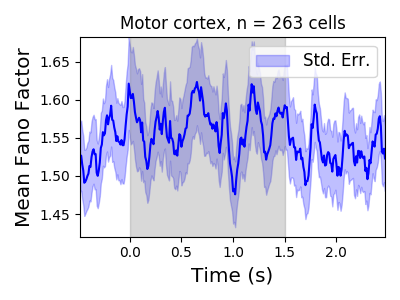
\includegraphics[width=\linewidth]{figures/conway_maxwell/motor_cortex_1ms_fano_factor.png}
      \caption{Motor cortex.}
      \label{fig:motor_cortex_fano_factor}
    \end{subfigure}
    \caption{(A) The mean Fano factor of the spike counts of the cells in the primary visual cortex. Means were taken across cells first, then across trials. There was a significant decrease in the Fano factors immediately after stimulus onset. (B) The mean Fano factor of the spike counts of the cells in the motor cortex. No significant change in measurements at any point.}
    \label{fig:fano_factors}
  \end{figure}

  Similar to these findings in the Fano factor, we found a reduction in the $\nu$ parameter of the COMB distribution on stimulus onset in V1 (figure \ref{fig:comb_nu_parameter}) and in no other region from which we had data. Specifically, the $\nu$ parameter reduced from around $1$, to between $1$ and $0$. This represents a change from no association between the neurons, to a positive association. It is possible that this positive association may be responsible for the reduction in the Fano factor.

\section{Discussion}
Our aim in this research was to develop a new statistical method for analysing the activity of a neuronal ensemble at very short timescales. We wanted our method to use information taken from the whole ensemble, but we also wanted the method to be quick and easy to implement. It is likely that analysis methods with these characteristics will become valuable as electrophysiological datasets include readings from more cells over longer time periods. In this case, we used the number of active, or spiking, neurons in a very short time bin ($<10$ms) as a measure of ensemble activity.

First of all, we showed that there were changes in response that we could model at these very short time scales in some of the brain regions from which we had recordings. We observed changes in the average number of active neurons, and the variance of the number of active neurons in three different brain regions in response to visual stimuli. Since we know that correlated behaviour is associated with sensory perception \parencite{decharms}, we might hope to measure the pairwise correlations within the neuronal population in order to further investigate these responses. But, using such short time bins can produce artificially small spike count correlation measurements \parencite{cohen1}. Overcoming this limitation was one of our objectives for our new method. In order to do this, we abandoned the idea of measuring the correlations directly and embraced the concept of \textit{association}. In order to quantify the association between neurons, we used the Conway-Maxwell-binomial distribution to model the number of active (spiking) neurons in an ensemble as a sum of possibly associated Bernoulli random variables.

We showed that the Conway-Maxwell-binomial distribution performed better than the more common options of the binomial and beta-binomial distributions. Furthermore, we showed that the positively associated behaviour between neurons in the primary visual cortex could be captured by fitting a Conway-Maxwell-binomial distribution, but was not captured by the more standard approach of measuring the spike count correlation. The associated behaviour could not be measured using spike count correlations, because of the very short bins required to capture short timescale behaviour.

We replicated a famous result from Churchland et al (2010) relating to the quenching of neural variability in cortical areas at stimulus onset, and in doing so, we established a correspondence between the association quantifying parameter of the Conway-Maxwell-binomial (COMb) distribution and the neural variability as measured by the Fano factor. We found a reduction in the $\nu$ parameter of the COMB distribution at stimulus onset, indicating a change from no association to positive association between neurons in V1. We found a corresponding reduction in the Fano factor of the individual cells in V1. The positive association between neurons induced by the stimulus would constrain the neurons to fire at the same time. The stimulus also induced a larger number of neurons to spike. These two actions combined could cause an increase in the firing rate of individual cells that is greater in magnitude than the increase in firing rate variability. If this is indeed the case, then the association as captured by the COMB distribution could be regarded as one of the `natural parameters' of the ensemble response for short timescales. That is, a quantity that directly measures some aspect of the behaviour of the ensemble. In this case, it the correlated behaviour of the individual neurons is captured.

This work could be just a first step in creating analysis methods based on the Conway-Maxwell-binomial distribution, or similar statistical models. One way to extend the method would be to pair it up with the `Population Tracking model' \parencite{odonnell}. This model attempts to characterise the interaction between an ensemble and each member of the ensemble by quantifying the probability of spiking for a given a cell, given the number of active cells in the whole population. Combining this model with the COMB distribution would give us a model that could accurately fit the number of active neurons at any moment, and that gives a probability of firing for each cell, and therefore probabilities for full spiking patterns, without adding a huge number of parameters to fit.

A more complex way to extend the model would be to fit a Conway-Maxwell-binomial distribution to data recorded from multiple brain regions simultaneously, with a different fit for each region, then to analyse the temporal relationship between the fitted parameters of each region. If we analysed the time series of the COMB distribution parameters from the different regions, looking at cross-correlations between regions, this may give some results relating to the timescales in which information is processed in different brain regions.

% TODO:   mention application to unsorted data
%         mention online applications

% Develop new method for analysing activity in neuronal ensemble
% We found that the Conway-Maxwell-binomial distribution was suitable for fitting to these data.
% We found that this was a good way to describe changes in association over a short timescale.
% Future work:  Pairing with population tracking model.
%               temporal element (shimazaki)
%                 Hierarchical element.
